%====================================================================================================
% Biblioteca Digital: Uma Estratégia de Gestão e Preservação de Periódicos do Século XX com DSpace e Metadados Dublin Core
%====================================================================================================
% TCC
%----------------------------------------------------------------------------------------------------
% Autor				: Vagner da Silva Bezerra
% Orientador		: Juliana Wolf Pereira
% Instituição 		: UFMS - Universidade Federal do Mato Grosso do Sul
% Departamento		: CPCX - Sistema de Informação
%----------------------------------------------------------------------------------------------------
% Data de criação	: 10 de Outubro de 2016
%====================================================================================================

\chapter{Metodologia} \label{cap:metodologia}

%Devido ao fato de haver bibliotecas que não passaram por nenhum tipo de teste de desempenho ou de funcionalidade. Ocorre muitas das vezes a existência de fahas causadas por leaks de memória, por exemplo, a biblioteca ConfigFile baixada do repositório do mbed. Essas falhas pode ser detectada pela ferramenta valgrind. Leaks de memória: invalid free, invalid write e invalide read. Citar dissertação Kleber.

Este trabalho teve como objetivo ampliar as bibliotecas \textit{FaultInjector} e \textit{FaultRecovery}, ambas desenvolvidas por Kruger \cite{Kruger:2014} em sua dissertação de mestrado. A biblioteca \textit{FaultInjector} possibilita a injeção de falhas no sistema mediante a simulação do fenômeno \textit{bit-flip} nas regiões da memória \textit{SRAM} do microcontrolador. Já a biblioteca \textit{FaultRecovery} proporciona o desenvolvimento de sistemas embarcados confiáveis, pois dispõe de técnicas de tolerância a falhas (baseadas na redundância de dados e de processamento) para aumentar a confiabilidade do sistema.

Foram utilizados exemplos variados para exemplificar as modificações realizadas na \textit{FaultRecovery}, pois se pensou em criar uma biblioteca genérica que possa ser utilizada em diversos casos, seja no sistema embarcado (\textit{firmware}) de um estacionamento, em um robô seguidor de linha ou em uma estação meteorológica.

%Como expansão ao trabalho de Kruger, foi melhorado o injetor de falhas de falhas na memória \textit{flash} da biblioteca \textit{FaultInjector} e a classe TData, responsável pela redundância de dados. A arquitetura da biblioteca também pode ser utilizada por sistemas de outras plataformas, por exemplo, os sistemas embarcados implementados para \textit{arduino} que são utilizados na área de robótica e são implementados por meio de máquina de estados.

Para a ampliação das biblioteca citadas, utilizou-se um microcontrolador de prototipagem rápida \textit{mbed}, modelo NXP LPC1768 \cite{lpc1768:2016} (o mesmo utilizado por Kruger). Este é projetado para a prototipagem de diversos equipamentos, especialmente aqueles que necessitam de conexão com a internet, portas USB e interfaces variadas para periféricos. Ele possui um núcleo ARM Cortex-M3 32 bits com 96 MHz de \textit{clock}, 64 KB de memória \textit{RAM} (32 KB disponíveis ao usuário e 32 KB reservados aos controladores internos do dispositivo), uma memória \textit{flash} de 512 KB, portas \textit{built-in Ethernet}, USB Host, CAN (\textit{Controller Area Network}), SPI (\textit{Serial Peripheral Interface}), I2C (\textit{Inter-Integrated Circuit}), ADC (\textit{Analog-to-Digital Converter}), DAC (\textit{Digital-to-Analog Converter}), PWM (\textit{Pulse-Width Modulation}) e outras interfaces de entrada e saída.

O \textit{mbed} também possui um temporizador \textit{watchdog}. Este componente consiste em um hardware responsável por reiniciar automaticamente o dispositivo em caso de falhas. O hardware temporizador é carregado com um valor inicial, decrementado a cada vez que o \textit{watchdog} é executado. Enquanto isso o programa principal executa em um \textit{loop}, repondo o temporizador a cada vez que passa pelo circuito principal. Se por conta de uma falha a reposição não ocorrer e o temporizador zerar, o dispositivo é reiniciado \cite{mbedWhatdog:2016}.

No sítio oficial da plataforma \textit{mbed} são fornecidas soluções para auxiliar no desenvolvimento de sistemas embarcados. Além da possibilidade de baixar bibliotecas fornecidas pela comunidade, o sítio disponibiliza um \textit{forum} para retirada de dúvidas. A \textit{mbed} também fornece um compilador online, com o qual após a compilação do código, um arquivo binário é gerado para ser executado no microcontrolador. Este compilador online tem a capacidade de compilar códigos para diversos modelos do \textit{mbed} \cite{mbedCompiler:2016}.

Além do modelo LPC1768, existem outros pertencentes à família \textit{mbed} NXP LPC17X, são eles: LPC1764, LPC1765, LPC1766 \cite{manualLpc176x:2016}. Embora apresentem arquiteturas compatíveis, o tamanho e o mapa de memória \textit{flash} e \textit{SRAM} varia conforme cada modelo, distinguindo-se por exemplo, nos modelos LPC1768/66/65 que possuem regiões de memória \textit{SRAM} nas mesmas faixas de endereço, mas diferentes do modelo LPC1764, conforme é mostrado na Figura \ref{Img:memoryMap} da seção a seguir.

%Nenhuma outra técnica, além do temporizador \textit{watchdog} foi utilizada para aumentar a confiabilidade do sistema \cite{Kruger:2014}.O Compilador online foi utilizado neste trabalho para criar a arquitetura para o desenvolvimento. Com o primeiro contato com o microcontrolador \textit{mbed} identificou-se a necessidade de estudar suas funcionalidades. Com a utilização do compilador online foi possível verificar que seria inviável adotá-lo como um editor de código para a expansão do injetor de falhas e da biblioteca \textit{faultRecovery}. A solução encontrada foi a utilização do ambiente de desenvolvimento integrado (IDE) LPCXpresso, pois o compilador online do \textit{mbed} permite exportar a arquitetura criada para essa IDE. O LPCXpresso é baseado na IDE eclipse e possui versões gratuitas e pagas, neste trabalho utilizou-se a versão gratuita para o modelo NXP LPC176. 

%, implementando um mapeamento do espaço de memória permitindo com que o injetor de falhas possa ser utilizado por qualquer modelo \textit{mbed} LPC176x, injeção de falhas na memória \textit{flash} e a ampliação da biblioteca \textit{faultRecovery} para implementação de sistemas embarcados por meio de máquinas de estados.

%Nenhuma outra técnica, além do temporizador \textit{watchdog} foi utilizada para aumentar a confiabilidade do sistema \cite{Kruger:2014}. dissertação de mestrado de Kruger \cite{Kruger:2014} o módulo \textit{GPS} não enviava dados para o servidor, sabendo-se que o microcontrolador \textit{mbed} pode se conectar a internet por meio desse módulo, a funcionalidade para enviar os dados coletados pela estação meteorológica será implementada nos próximos meses de execução deste trabalho, atualmente a biblioteca \textit{GPS} está com um erro de programação que fixa a execução do código em um loop infinito.


\section{Injetor de Falhas} \label{sec:InjetorDeFalhas}

A injeção de falhas é um processo importante para validar e verificar a confiabilidade de um sistema, seja por alteração de código, simulando uma falha de \textit{software} ou a nível de pinos (\textit{Pin-level Injection}), injetando falhas diretamente no hardware. A biblioteca \textit{FaultInjector} permite simular o efeito do \textit{bit-flip} em qualquer região de memória \textit{SRAM} do microcontrolador \textit{mbed} LPC1768, mas apresenta duas graves limitações: a falta de flexibilidade, por não executar em outros modelos de microcontroladores, e a impossibilidade de inserção de falhas nas regiões da memória \textit{flash}. Essas limitações são descritas respectivamente nas subseções \ref{subsec:MapDeMemoria} e \ref{subsec:InjecaoFalhasFlash}.

\subsection{Mapeamento de Memória} \label{subsec:MapDeMemoria}

Inicialmente, pensou-se em ampliar o uso da biblioteca \textit{FaultInjector} mediante a criação de várias versões, cada uma específica a um modelo da família LPC176X. Assim, o programador ficaria responsável por baixar a versão correta. Entretanto, conforme as pesquisas evoluíram, percebeu-se que era possível identificar dentro do próprio código-fonte o modelo do microcontrolador, uma vez que o compilador mantém a informação do modelo em uma \textit{define} \footnote{Constante}. Com esta descoberta, foi possível criar uma única versão que automaticamente mapeia as regiões de memória.

Neste primeiro passo, observando o mapa de memória da família \textit{mbed} LPC176X \cite{manualLpc176x:2016} foi possível constatar que alguns modelos possuem regiões de memória idênticas, conforme mostrados na Figura \ref{Img:memoryMap}. Logo, o uso de heranças e classes abstratas poderiam ser utilizadas com o intuito de facilitar o mapeamento das regiões de memória e promover uma interface à biblioteca \textit{FaultInjector}, que precisava injetar falhas nas regiões de memória sem necessariamente conhecer os endereços das regiões de cada dispositivo.

Com as regiões de memória mapeadas, o segundo passo foi a implementação desse mapeamento. A classe \textit{MemoryRegion}\cite{Kruger:2014} foi utilizada para representar as regiões de memória do \textit{mbed}. Ela contém atributos que armazenam o endereço de memória inicial, o endereço final e o tamanho (em bytes) de cada região de memória. 

A classe abstrata \textit{MemoryMap} representa o mapa de memória de um microcontrolador \textit{mbed} e disponibiliza uma interface para \textit{FaultInjector} injetar falhas. Esta classe é herdada por classes não-abstratas, como a classe \textit{MemoryMap\_LPC1764} e \textit{MemoryMap\_LPC1768}, que obrigatoriamente, ficam responsáveis por implementar os métodos abstratos \textit{getUserMemoryRegion()} e \textit{getFlashMemoryRegion()} de \textit{MemoryMap}, descritos a seguir:

\begin{itemize}
	\item \textbf{\textit{getUserMemoryRegions()}} - método abstrato que retorna uma lista das regiões de memória disponíveis para o usuário.				
	
	\item \textbf{\textit{getFlashMemoryRegions()}} - método abstrato que retorna a lista de regiões endereçadas a memória \textit{flash}.
	
	\item \textbf{\textit{getPeripheralsMemoryRegions()}} - retorna uma lista de regiões da memória destinadas aos periféricos. Este método não é abstrato, mas pode ser sobrescrito. Entretanto, como as regiões dos periféricos do microcontrolador é comum a todos eles, não há necessidade alguma sobrescrever este método.
\end{itemize}

Pela \textit{FaultInjector} ser capaz de identificar o modelo do microcontrolador, ela mesma é responsável por escolher qual das versões de \textit{MemoryMap} irá utilizar (\textit{MemoryMap\_LPC1764}, \textit{MemoryMap\_LPC1765}, entre outros). Isso tornou a biblioteca flexível, sendo possível injetar falhas nos nas regiões de memória mostradas na Figura \ref{Img:memoryMap}. A biblioteca está disponível no endereço \url{https://github.com/cleitonalmeida1/FaultInjector}.

\begin{figure}[H]
	\centering
	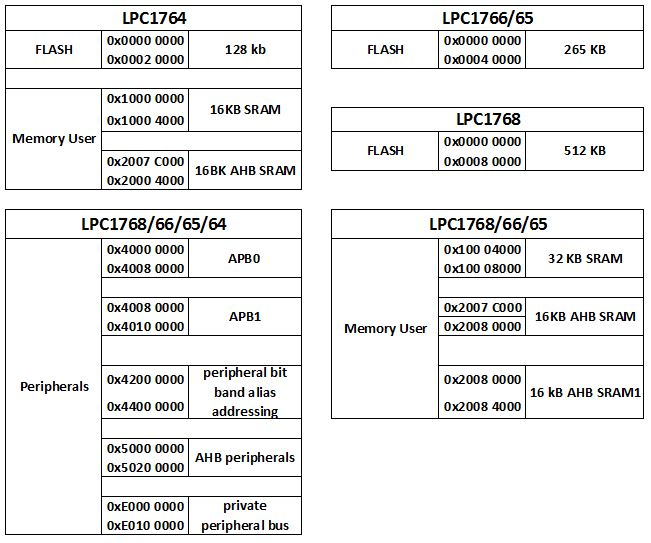
\includegraphics[width=1.0\textwidth]{figuras/memoryMap.jpg}
	\caption[Mapas das Regiões de Memória dos Modelos LPC1768/66/65/64]{Mapeamento das regiões de memória dos modelos LPC1768/66/65/64.}
	\label{Img:memoryMap}	
	%width=0.5\textwidth (Tamanho da Imagem)
\end{figure}


\subsection{Injeção de Falhas na Memória Flash} \label{subsec:InjecaoFalhasFlash}

Os microcontroladores \textit{mbed} possuem memória \textit{flash}, na qual o código do \textit{firmware} é armazenado \cite{manualLpc176x:2016}. Logo, a alteração de um único bit em um endereço de memória que contenha partes de uma instrução pode resultar em um falha irreversível. No entanto os dados coletados por um sistema também podem ser armazenados na memória \textit{flash}. Considerando-se o sistema embarcado de uma estação meteorológica que precisa coletar os dados climáticos e armazená-los na memória não volátil. Estes dados armazenados na \textit{flash} são enviados a um servidor remoto após um período de tempo predefinido. Se um único bit da região de memória na qual os dados coletados estão armazenados for alterado (\textit{bit-flip}), esta alteração poderá provocar uma modificação no valor da informação armazenada que poderia ser, por exemplo, um valor da umidade do ar, que perderia a exatidão após sua alteração, ou seja, o dado coletado enviado para o servidor remoto estaria incorreto, impactando em uma equivocada previsão do tempo. 

Conforme explicado na Seção \ref{sec:InjecaoDeFalhas}, um dos aspectos positivos na simulação de falhas por software é a segurança de não danificar o dispositivo. Falhas podem ser inseridas em bytes aleatórios na memória \textit{SRAM} simulando o fenômeno \textit{bit-flip}, entretanto, a mesma lógica não pode ser aplicada na memória \textit{flash}, pois por ser protegida não é possível escrever um único endereço de memória, somente a escrita por setores que são no total 29, divididos em duas áreas. A primeira, que abriga os setores do 1 ao 15 contém blocos de 4KB, a segunda, que vai do setor 16 até o 29, é composta por blocos de 32KB para cada setor \cite{manualLpc176x:2016}.

A injeção de falhas na \textit{flash} foi realizada mediante a escrita de bytes em um setor de memória sorteado aleatoriamente. Foram copiado 256 bytes da memória \textit{SRAM}, que é a quantidade mínima de bytes que podem ser escritos com a biblioteca retirada do repositório de bibliotecas da \textit{mbed} \cite{escritaNaFlash:2016}, para a \textit{flash} utilizando uma biblioteca que permite fazer operações na memória não volátil. 

Para realizar a injeção de falhas na flash foi necessário seguir os seguintes passos:

\begin{itemize}
	\item Sortear um setor aleatório da memória flash.
	
	\item Copiar a quantidade de bytes escolhida da memória \textit{RAM} podendo variar entre 256, 512, 1024 ou 4096.
	
	\item Preparar o setor para escrever os bytes copiados da memória \textit{RAM} determinando qual o número do setor inicial e qual o do setor final.
	
	\item Após a delimitação do setor inicial e final a escrita dos bytes copiados da memória serão escritos na flash.
	
\end{itemize}

Neste trabalho foi realizada a escrita de 256 bytes na memória \textit{flash}, ou seja, foram injetadas 256 bytes de falhas em setores aleatórios. As regiões da \textit{flash} armazenam dados estáticos e as instruções do programa, logo, falhas nesses setores podem causar uma falha irreversível no sistema afetando o seu correto funcionamento. Porém a injeção de falhas não foi realizada durante a execução de algum programa, pois faltou tempo hábil e o interesse era explorar a memória \textit{flash} ou seja, descobrir se seria possível injetar falhas nessa região de memória, uma vez que quando Kruger \cite{Kruger:2014} tentou injetar falhas na memória \textit{flash}, o microcontrolador travava durante a execução do injetor.

\section{FaultRecovery: Extensão da biblioteca} \label{sec:extensaoBiblioteca}

Inicialmente pensou-se em ampliar a biblioteca \textit{FaultRecovery} utilizando a sua estrutura inicial, que implementa macros e funções de \textit{callback} (função executada conforme a ocorrência de um evento predefinido). No entanto, o uso de macros como funções não é uma boa prática de programação \cite{Meyers:2011}, pois além de dificultarem o entendimento da estrutura do código, criam outros males que podem resultar em falhas inesperadas. Por exemplo, uma macro que chama uma função \textit{f} para que se retorne o maior entre os argumentos, se chamada com um dos parâmetros sob incremento, pode gerar erros imprevistos, conforme mostram os Quadros \ref{Func:Macro} e \ref{Func:MacroInvocacao}.

\begin{lstlisting}[label=Func:Macro,caption={[Uso de macro como função] Macro que chama \textit{f} como o máximo entre a e b}]
#define CALL_WITH_MAX(a, b) f((a) > (b) ? (a) :(b))
\end{lstlisting}

\begin{lstlisting}[label=Func:MacroInvocacao,caption={[Macro sendo chamada no código] Na primeira invocação da macro a variável a é incrementada duas vezes e na segunda uma vez.}]
int a = 5, b = 0;
CALL_WITH_MAX(++a, b);
CALL_WITH_MAX(++a, b + 10);
\end{lstlisting}

%Utilizou-se o exemplo anterior escrito por Meyers \cite{Meyers:2011} para ilustrar uma das desvantagens de se implementar macros na expansão da biblioteca \textit{FaultRecovery}.

Na \textit{FaultInjector} de Kruger, as macros eram utilizadas demasiadamente, por isso foram substituídas por funções \textit{templates}. Outra modificação importante foi o emprego do padrão de projeto \textit{State}. Esse é indicado para programas que implementam máquinas de estados e teve como objetivo facilitar o uso da biblioteca, pois trouxe uma estrutura capaz de gerenciar automaticamente as mudanças de estados.

\subsection{Refatoração e Aperfeiçoamento: Versão 1.0} \label{subsec:versao1}

O emprego do padrão de projeto \textit{State} na refatoração da biblioteca, tem como um de seus principais objetivos forçar o usuário a implementar seu \textit{firmware} como uma máquina de estados. Embora todo \textit{firmware} seja uma máquina de estados, a maioria deles não são orientados a objetos e tão pouco legíveis. Foi Implementada uma versão dessa biblioteca para \textit{arduino} e está sendo utilizada no projeto de extensão Coxim Robótica, do Campus de Coxim - UFMS para o desenvolvimento de um carrinho seguidor de linha. Na Figura \ref{Img:diagramaFaultRecovery} é mostrado o diagrama de classes da biblioteca \textit{FaultRecovery}.

\begin{figure}[H]
	\centering
	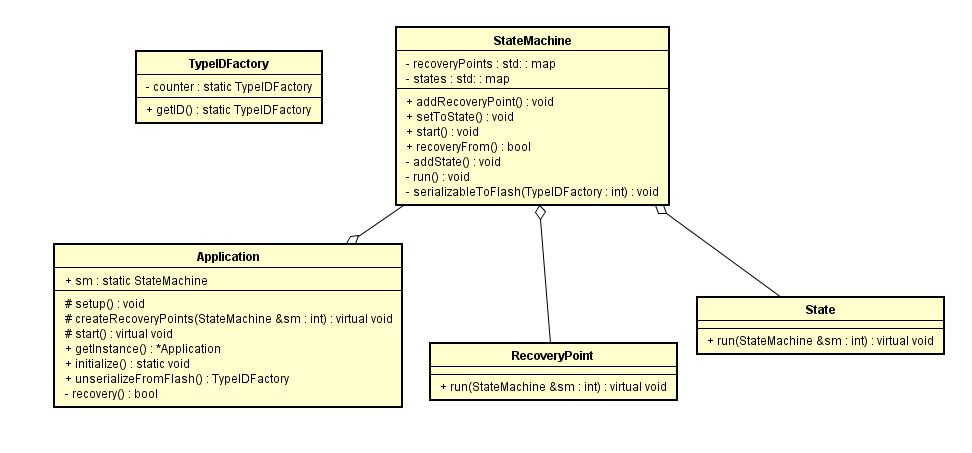
\includegraphics[width=0.9\textwidth]{figuras/diagramaFaultRecovery.jpg}
	\caption[Diagrama de classes da biblioteca \textit{FaultRecovery}.]{Diagrama de classes da biblioteca \textit{FaultRecovery}.}
	\label{Img:diagramaFaultRecovery}	
	%width=0.5\textwidth (Tamanho da Imagem)
\end{figure}

O uso do padrão de projeto mencionado e a aplicação dos conceitos de orientação a objetos possibilitou a criação de programas modularizáveis, em outras palavras, o código do \textit{firmware} pode ser separado por responsabilidades. Cada estado contém a sua classe de implementação, permitindo a separação do código e facilitando o entendimento da equipe. A primeira versão da biblioteca possuia três classes: \textit{TypeIDFactory, State} e \textit{StateMachine}, descritas abaixo:

\begin{itemize}
	\item \textit{\textbf{TypeIDFactory}} - Esta classe é responsável pela geração dos IDs de identificação dos estados. Os identificadores são únicos e auto-incrementais. Estes IDs são utilizados para indexar os estados em um \textit{hash map}.
	
	\item \textit{\textbf{State}} - Esta classe é responsável pela representação de um estado. Composta por um método abstrato \textit{run}, é a classe base para todos os estados do \textit{firmware}. No método \textit{run} o usuário implementa as rotinas de execução do estado. Caso ao final dessa rotina haja uma transição para um novo estado, o método \textit{setToState} deve ser invocado passando entre os sinais ($<$ $>$) a classe que representa o próximo estado a ser executado, conforme demonstrado no \autoref{Func:faultRecovery}. Apenas a classe é passada como parâmetro do \textit{template}, uma vez que a própria \textit{StateMachine} é responsável pela alocação dos objetos em seu \textit{hash map}. Essa abordagem evita cópias desnecessárias e perda de desempenho.
	
	\item \textit{\textbf{StateMachine}} - Esta classe representa a máquina de estados e tem a responsabilidade de controlar o despacho das funções implementadas em cada estado. Funciona como uma espécie de ``engrenagem'', que controla as transições entre os diversos estados do sistema, instanciando e adicionando os novos estados em um \textit{hashmap} e selecionando-os a cada transição do programa. A escolha de um \textit{hash map} deveu-se ao seu desempenho ser superior a outras estruturas de dados, uma vez que os estados são indexados pelos seus IDs.
	
	Conforme mostrado na Figura \ref{Img:fluxoFaultRecovery} no momento em que o programa recebe um evento responsável pela mudança de estado, o método \textit{setToState} desta classe recebe o valor da variável \textit{current} (determina o estado atual). Se o estado não estiver sido adicionado no \textit{map} de estados da máquina de estados, o método \textit{addState} será chamado para incluir esse novo estado.
	
	 Para executar a máquina de estados, deve-se instanciar um objeto \textit{StateMachine} e chamar o método \textit{start}, passando entre ($<$ $>$) o estado inicial conforme demonstrado no \autoref{Func:faultRecovery}, o método \textit{start} chamará o método \textit{setToState} e o método \textit{run}. Este Executará a máquina de estados por meio de um \textit{loop}. Aquele atribuirá o id do estado inicial para a variável \textit{current}.
		
\end{itemize}

\begin{figure}[H]
	\centering
	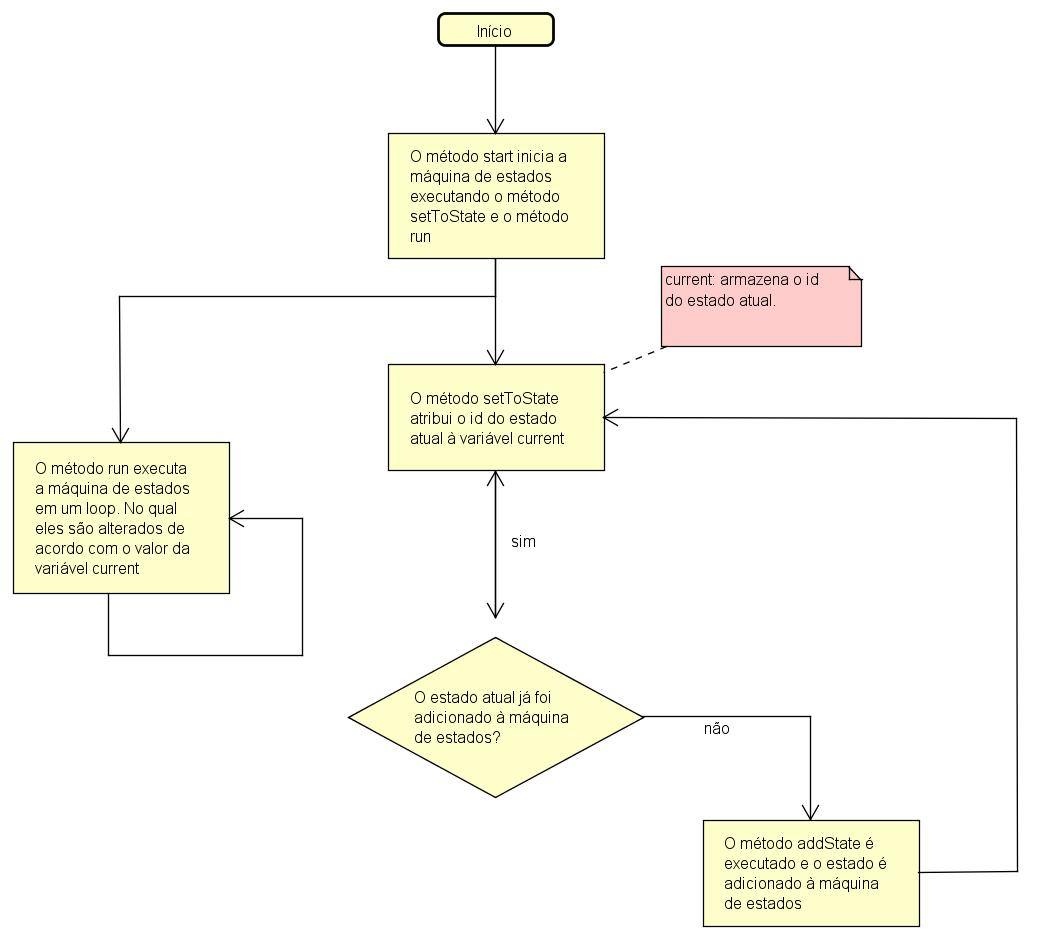
\includegraphics[width=0.9\textwidth]{figuras/fluxoFaultRecovery.jpg}
	\caption[Fluxograma da biblioteca \textit{FaultRecovery}.]{Fluxograma da biblioteca \textit{FaultRevorery}.}
	\label{Img:fluxoFaultRecovery}	
	%width=0.5\textwidth (Tamanho da Imagem)
\end{figure}
\newpage
\begin{lstlisting}[label=Func:faultRecovery,caption={[Exemplo de criação de um estado]A classe EsperandoCarroChegar herda da classe \textit{State} e tem sua rotina implementada no método \textit{run}, ao encerrar a rotina o método \textit{setToState} é invocado, alterando o estado atual. No método \textit{main} um objeto \textit{StateMachine} é instanciado e o método \textit{start} é chamado, iniciando a máquina de estados. Este quadro tem como objetivo demonstrar a utilização da biblioteca, apenas um estado será posto no quadro, os demais podem ser acessados no endereço \url{https://github.com/cleitonalmeida1}.}]
	class EsperandoCarroChegar: public State {
		void run(StateMachine &sm) {
			if (carroChegou()) {
				sm.setToState<EsperandoApertarBotao>();
			}
		}
	};
		int main() {
		StateMachine sm;
		sm.start<EsperandoCarroChegar>();
	}
\end{lstlisting}

Um exemplo simples para ilustrar a utilização da nova \textit{FaultRecovery} é o programa de estacionamento de um shopping. A entrada do estacionamento possui um emissor de \textit{tickets}, dois sensores e uma cancela. Ao se aproximar da cancela, o motorista aperta um botão para emitir um \textit{ticket}, após a emissão a cancela é aberta, os sensores detectam a entrada do carro ao interior do estacionamento e a cancela é fechada.

A máquina de estados do caso ilusório é composta por quatro estados, um deles é demonstrado no \autoref{Func:faultRecovery}:

\begin{itemize}
	\item \textbf{EsperandoCarroChegar} - Este é o estado inicial da máquina de estados. O sensor de presença detecta a chegada do veículo na entrada do estacionamento, o carro se aproxima da entrada, então o estado EsperandoCarroChegar detecta a aproximação do veículo e chama o próximo estado.
	
	\item \textbf{EsperandoApertarBotao} - Neste estado o dispositivo eletrônico emite o \textit{ticket} de estacionamento após o motorista apertar o botão. Após isso, o estado atual é alterado para EsperandoCarroEntrar. Outra situação é quando o motorista decide não adentrar ao estacionamento, neste caso o estado é alterado para o anterior (EsperandoCarroChegar). 
	
	\item \textbf{EsperandoCarroEntrar} - Neste estado os sensores estão aguardando a entrada do carro ao estacionamento. O sensor externo ao estacionamento detecta duas situações, a primeira é quando o carro se afasta da cancela e não entra no estacionamento, neste caso a máquina de estados retorna ao seu estado inicial. O segundo é quando o carro adentra ao estacionamento, neste caso o sensor externo identifica a entrada do carro, o interno ao estacionamento detecta o carro se afastando da cancela, com o seu afastamento o sistema altera o estado para FecharCancela.
	
	\item \textbf{FecharCancela} - Neste estado o carro se afasta da entrada do estacionamento, o sensor externo a esse detecta o afastamento do carro e a cancela é fechada. Ao fechar a cancela o estado FecharCancela, por ser o último estado da máquina de estados, irá chamar o estado inicial, para então reiniciar o ciclo de execução dos estados.
	
\end{itemize}


\subsection{Refatoração e Aperfeiçoamento: Versão 2.0} \label{subsec:versao2}

Na Subseção \ref{subsec:versao1} que trata da versão 1.0 da biblioteca, mostrou-se como implementar os estados de uma máquina de estados. Esta subseção trata da criação dos pontos de recuperação, como inicializar a máquina de estados e quais as classes adicionadas na biblioteca e suas responsabilidades. Nesta etapa de desenvolvimento, focou-se na tolerância a falhas. A versão 2.0 da biblioteca \textit{FaultRecovery} utiliza a máquina de estados desenvolvida na versão 1.0, no entanto foi adicionada a funcionalidade que possibilita a criação de pontos de recuperação de falhas. Se o microcontrolador trava durante a execução da máquina de estados, o defeito é detectado pelo \textit{whatchdog}, já que o temporizador tem seu valor de limiar excedido, e então o \textit{whatchdog} reinicia o dispositivo. Ao restaurar, é possível diagnosticar o último estado seguro, pois esta informação foi gravada na \textit{flash} durante as trocas de estado. Caso exista algum ponto de recuperação configurado para este último estado seguro, será executado. 

O usuário da biblioteca deve criar os pontos de recuperação conforme seja necessário, sendo possível adicionar no máximo um ponto de recuperação por estado. Estes pontos indicam quais as rotinas deverão ser executadas caso o programa falhe durante a execução do estado especificado. Essa rotina pode executar uma determinada configuração no microcontrolador ou uma tarefa que deva ser iniciada antes da máquina de estados ser inicializada.

As classes \textit{Application} e \textit{RecoveryPoint} foram adicionadas à biblioteca. A primeira é responsável pela inicialização do \textit{firmware} e gerenciamento dos pontos de recuperação, a segunda é responsável pela implementação dos pontos de recuperação. Para utilizar a versão 2.0, deve-se instanciar um objeto \textit{Application} e chamar o método \textit{initialize} da seguinte forma: Application:initialize$<$EstacionamentoApp$>$. A classe EstacionamentoApp é herdada de \textit{Application}, que possibilita a implementação de três métodos, sendo o método \textit{start} obrigatório (pois é puramente virtual) e os métodos \textit{creatRecoveryPoints} e \textit{setup} opcionais (pois não são puramente virtuais). O método \textit{initialize} é \textit{static}, ou seja, ele pode ser chamado a partir de um código externo à classe sem a necessidade de criar uma nova instância de \textit{Application}. Ao evocar o método \textit{initialize}, um objeto \textit{StateMachine} é inicializado, uma instância da classe EstacionamentoApp também é inicializada, essa será utilizada durante toda a execução da máquina de estados. Após o EstacionamentoApp ser inicializado, quatro métodos serão evocados automaticamente. 

O primeiro é o método \textit{setup} que poderá ou não ser implementado. Neste método são implementadas as configurações do microcontrolador, que podem variar dependendo do seu modelo, vale ressaltar que a utilização desta biblioteca não se limita ao microcontrolador \textit{mbed}, pois os extensionistas do projeto Coxim Robótica do Campus de Coxim - UFMS já estão utilizando a arquitetura da biblioteca \textit{FaultRecovery} adaptada para a plataforma \textit{arduino}, por exemplo, no método \textit{setup} os extensionistas programaram as configurações iniciais de um robô seguidor de linha e cada aluno ficou responsável por implementar um estado da máquina de estados do carrinho.

O segundo é o método \textit{createRecoveryPoints}, que poderá ou não ser implementado, pois por padrão esse método não adiciona nenhum ponto de recuperação à máquina de estados. Entretanto pode ser sobrescrito, caso necessário, para que pontos de recuperação sejam adicionados à máquina de estados. Para implementar um ponto de recuperação deve-se criar uma classe que herde de \textit{RecoveryPoints}. 

Ao herdar dessa classe, o usuário obrigatoriamente deverá implementar o método abstrato \textit{run} no qual conterá as rotinas de execução caso o programa seja restaurado daquele ponto. Para adicionar um ponto de recuperação à máquina de estados, deve-se utilizar o método \textit{addRecoveryPoint} nativo da classe \textit{StateMachine} e evocá-lo conforme demonstrado no quadro \autoref{Func:addRecoveryPoint}. Esse receberá entre $< >$ o ponto de recuperação e o estado ao qual ele pertence, sendo assim o ponto de recuperação fica associado ao estado, em outras palavras, o id de identificação do estado no \textit{hashmap} de estados será o mesmo do seu ponto de recuperação no \textit{hashmap} de pontos de recuperação.

Como mencionado, na versão 2.0 o método \textit{setToState} da classe \textit{StateMachine} além de trocar o estado atual, também armazena o seu id na memória flash do microcontrolador \textit{mbed}. Quando o dispositivo for reiniciado, se existir um ponto de recuperação para o id armazenado na memória \textit{flash} a biblioteca executará o ponto de recuperação referente ao id lido da memória \textit{flash}.

O terceiro é o método \textit{start} no qual é realizada a inicialização da máquina de estados conforme demonstrada no segundo parágrafo desta Subseção.

\begin{lstlisting}[label=Func:addRecoveryPoint,caption={[Métodos \textit{createRecoveryPoints} e \textit{run}]Este quadro demonstra a implementação do método \textit{createRecoveryPoints} implementado no EstacionamentoApp que herda de \textit{Application}. O ponto de recuperação é criado quando o método \textit{addRecoveryPoint} é evocado, percebe-se que existem duas classes separadas por vírgula e entre $<$$>$, a primeira é a implementação do ponto de recuperação, ou seja, a classe que herda de \textit{RecoveryPoints}. A segunda é a classe que representa o estado que deverá ser executado após a reinicialização do microcontrolador, ou seja, caso ele inicie neste ponto de recuperação o estado EsperandoCarroEntrar deverá ser escutado. No método \textit{run} da classe RecoveryEsperandoCarroEntrar encontra-se o código que será executado caso o microncontrolador falhe no momento em que o carro iria entrar no estacionamento. Se a energia acabasse durante o fechamento da cancela e o programa tivesse voltado com a cancela aberta, o dono do estacionamento teria prejuízo, pois alguns carros poderiam entrar sem pagar a taxa de estacionamento enquanto a cancela estivesse aberta.}]
	//Estacionamento App Class
	void EstacionamentoApp::createRecoveryPoints(StateMachine &sm) {
		sm.addRecoveryPoint<RecoveryFecharCancela, FecharCancela>();
	}

	//RecoveryFecharCancela Class
	void RecoveryFecharCancela::run(StateMachine &sm) {
		if (checarPortaoAberto()) {
			fecharPortao();
		}
		sm.start<EsperandoCarroEntrar>();
	}
\end{lstlisting}

\newpage

\section{\textit{Classe de Redundância de Dados: TData}} \label{sec:classeTData}

A classe \textit{TData} foi implementada com o objetivo de obter-se uma redundância de dados automatizada, tanto para variáreis primitivas (int, float, long, double, char, bool), quanto para objetos de uma classe. Existem duas maneiras de se criar um objeto \textit{TData}, a primeira é utilizando tipos primitivos e a segunda objetos. 

Ao instanciar um objeto \textit{TData}, deve-se especificar o seu tipo e passar um valor ou um objeto no construtor: TData$<$tipo\_da\_variável$>$ variavel(valor). Ou o valor, ou o objeto passado como parâmetro serão copiados para três cópias de segurança, das quais serão utilizadas para manter a integridade do valor original por meio de um sistema de votação, que verifica se os valores das cópias são consistentes.

\subsection{Classe TData com Tipos Primitivos} \label{subsec:TDataPrimitivo}

O método \textit{setData} (pertencente a classe \textit{TData}) será invocado automaticamente ao passar o número inteiro 4 como parâmetro no construtor da classe. Ao alterar o valor 4 para a operação 1 + 9, o método \textit{setData} será implicitamente chamado por meio de sobrescrita de operadores, disponível na linguagem C++, possibilitando que o valor da variável seja atualizado juntamente com as cópias de segurança. Vale ressaltar que a cada vez que o objeto \textit{TData} for acessado, o método \textit{getByVotting()} que implementa um esquema de votação será executado, validando todas as cópias do objeto \textit{TData}. A injeção de falhas foi realizada por meio do método temporário chamado \textit{injectFault}, que modificou o valor de uma das cópias do objeto \textit{TData}, simulando o fenômeno \textit{bit-flip}. Esse método foi utilizado durante a implementação da classe \textit{TData}, sendo retirado dela após sua conclusão. Na Figura \ref{Img:tdataPrimitivo} é mostrado os valores das cópias após a injeção de falhas.

\begin{figure}[H]
	\centering
	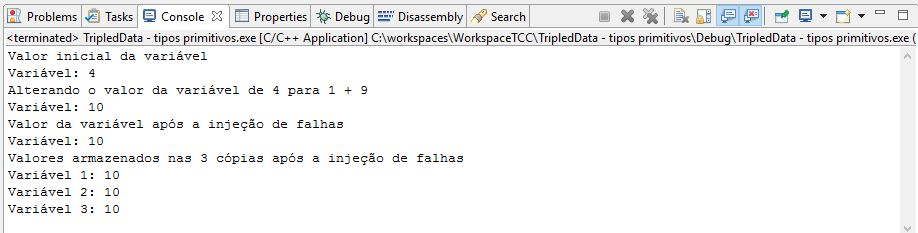
\includegraphics[width=1.0\textwidth]{figuras/tdataPrimitivo.jpg}
	\caption[Figura que apresenta a saída com os valores das cópias consistentes para tipos primitivos após a injeção de falhas.]{Nesta figura é mostrado que o valor das cópias foram atualizados após a operação 1 + 9. Também é mostrado que os valores das cópias continuaram consistentes após a injeção de falhas.}
	\label{Img:tdataPrimitivo}	
	%width=0.5\textwidth (Tamanho da Imagem)
\end{figure}	


\subsection{Um Exemplo Ilusório Para Utilização da Classe TData com Objetos} \label{subsec:exemploTData}

Para demonstrar como utilizar e instanciar a classe \textit{TData} com objetos, foi utilizado um exemplo que permitiu a utilização de objetos heterogêneos, ou seja, objetos que possuem outros objetos dentro de si, que podem ser objetos de pilha ou ponteiros para um endereço de memória. Destaca-se, um caso ilusório de um automóvel inteligente interligado a diferentes tipos de dispositivos e formas de comunicação, comunicando-se a um servidor. 

As informações disponibilizadas pelo veículo são navegação, diagnósticos do funcionamento do próprio veículo, dentre outras informações. Este por sua vez sofre um acidente e o sistema se encarrega de acionar outro sistema, ou seja, o sistema embarcado instalado no carro se comunica com outro remotamente. Este, por sua vez, receberia todos os dados relativos ao paciente, inclusive sua localização para um possível deslocamento de ambulâncias \cite{Valderi:2008}. Este exemplo foi implementado de maneira simples com o objetivo de demonstrar como instanciar e utilizar a classe \textit{TData}. 

Foram criadas duas classes para compor o cenário, sendo elas as classes Carro e Emergência, essas classes tiveram seus operadores de igualdade implementados pois, a classe \textit{TData} obriga que suas implementações sejam realizadas, visto que o compilador não é capaz de definir o comportamento de uma definição de igualdade em um objeto. Cada objeto define a igualdade de um jeito diferente, a classe \textit{string} por exemplo, define que igualdade são objetos com o mesmo conteúdo, ainda que sejam objetos distintos, ou seja, em endereços de memória diferentes.

A implementação dos operadores de igualdade para tipos primitivos não é obrigatória pois são tipos homogêneos, já os objetos podem ter outros objetos em seu escopo, como é o exemplo da classe Carro, que contém uma instância da classe Emergência em seu escopo, tornando obrigatória a implementação de seus operadores de igualdade, para que possam ser utilizados na classe \textit{TData}.

\subsection{Classe Carro com Objeto de Pilha} \label{subsec:classeObjetoPilha}

Para instanciar um objeto \textit{TData} do tipo Carro, primeiro deve-se declarar um objeto carro e setar os valores de seus atributos e consecutivamente instanciar um objeto \textit{TData} do tipo carro passando o objeto carro recém criado como parâmetro no construtor da classe com os seus valores preenchidos. 

Para este exemplo utilizou-se as classes Carro e Emergencia mencionadas nas Seções anteriores e o método \textit{injectFault} utilizado para simular o fenômeno \textit{bit-flip}. A injeção de falhas foi realizada com métodos temporários implementados dentro da classe \textit{TData} alterando os valores do telefone do hospital pertencente a classe Emergencia e da localização do carro pertencente a classe Carro.

O carro possui um sistema inteligente interligado com outros sistemas, ao sofrer o acidente automaticamente o sistema embarcado instalado no carro iria se conectar a outro sistema pedindo socorro e enviando sua localização para o hospital, essa por sua vez poderia ser alterada por alguma falha em seu endereço de memória podendo causar a morte do motorista, pois a ambulância seria enviada para outro endereço que não fosse o do carro. Após a injeção de falhas, os valores  de todas as cópias podem ser visualizados na Figura \ref{Img:tdataObjetoPilha} demonstrando que mesmo após a ocorrência de falhas nos endereços de memória da localização e do telefone do hospital, as cópias continuaram consistentes.

\begin{figure}[H]
	\centering
	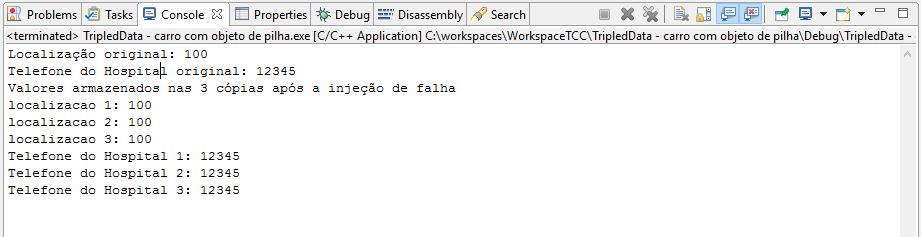
\includegraphics[width=1.0\textwidth]{figuras/tdataObjetoPilha.jpg}
	\caption[Valores das cópias consistentes após a injeção de falhas com objeto de pilha.]{Nesta figura é mostrado que valores das cópias continuaram consistentes após a injeção de falhas.}
	\label{Img:tdataObjetoPilha}	
	%width=0.5\textwidth (Tamanho da Imagem)
\end{figure}

\subsection{Classe Carro com Ponteiro} \label{subsec:CarroPonteiro}

Este parágrafo tem por objetivo demonstrar que a classe \textit{TData} também funciona com ponteiros. A classe \textit{TData} também pode receber como parâmetro em seu construtor objetos que contenham referência para endereços de memória. Realizou-se uma injeção de falhas no ponteiro emergencia (armazena o telefone do hospital), alterando o seu endereço de memória por meio do método \textit{injectFault}. Os valores do telefone e da localização após a injeção de falhas é mostrado na Figura \ref{Img:tdataPonteiro}, mostrando que mesmo após a modificação do endereço de memória do ponteiro emergência em uma das cópias, o valor do telefone do hospital continua o mesmo para todas as cópias.

\begin{figure}[H]
	\centering
	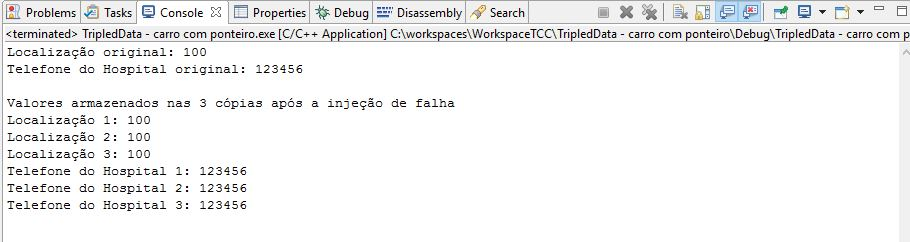
\includegraphics[width=1.0\textwidth]{figuras/tdataPonteiro.jpg}
	\caption[Valores das cópias consistentes após a injeção de falhas com ponteiro.]{Nesta figura é mostrado que os valores das cópias continuaram consistentes após a injeção de falhas.}
	\label{Img:tdataPonteiro}	
	%width=0.5\textwidth (Tamanho da Imagem)
\end{figure}

Além das três cópias de segurança que compõem a classe \textit{TData} existe mais uma cópia chamada \textit{dataObject}, utilizada para atualizar o objeto \textit{TData} sem a necessidade de passar o objeto modificado como parâmetro no construtor da classe. A variável \textit{dataObjet} é utilizada para replicar uma alteração no objeto para as demais cópias. Para acessar o objeto \textit{dataObject} é necessário chamar o método \textit{getDataObject} implementado para atualizar as três cópias e executar o método \textit{getByVotting} para manter a consistência de todas as cópias. Na Figura \ref{Img:tdataSetando} é mostrada a atualização do telefone do hospital e os valores das cópias após a injeção de falhas.

\begin{figure}[H]
	\centering
	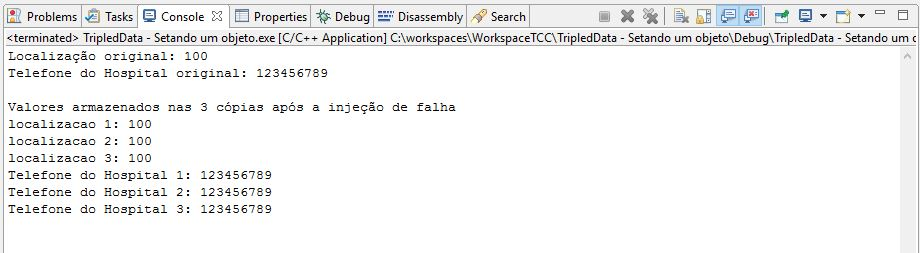
\includegraphics[width=1.0\textwidth]{figuras/tdataSetando.jpg}
	\caption[Figura que apresenta a saída com os valores das cópias consistentes após a atualização do objeto \textit{TData} do tipo carro e da injeção de falhas.]{Figura que apresenta a saída com os valores das cópias consistentes após a atualização do objeto \textit{TData} do tipo carro e da injeção de falhas.}
	\label{Img:tdataSetando}	
	%width=0.5\textwidth (Tamanho da Imagem)
\end{figure}